\renewcommand{\NomeBloco}{\textit{APS}}
\renewcommand{\NomeBlocoNoUnderline}{blocoAPS}
\renewcommand{\NomePTab}{tab_\NomeBlocoNoUnderline}
\renewcommand{\NomeSTab}{tab_\NomeBlocoNoUnderline2}
\renewcommand{\NomePFig}{fig_\NomeBlocoNoUnderline}
\renewcommand{\NomeSFig}{fig_\NomeBlocoNoUnderline2}
\renewcommand{\NomeTTab}{tab_\NomeBlocoNoUnderline3}
\renewcommand{\NomeQTab}{tab_\NomeBlocoNoUnderline4}

\section{APS}

O bloco \NomeBloco{} implementa o circuito apresentado na \autoref{fig_APS}. O bloco apresenta as definições de sinais de entrada e sa\'ida referidos na \autoref{\NomeSTab}.

\begin{table}[!h]
\caption{Sinais do bloco \NomeBloco}
\label{\NomeSTab}
\centering
\begin{tabular}{ccll}

    \toprule
    Sinal & Tipo    & Descrição & Observação        \\
    \midrule \midrule
    RESET   & Entrada   & Sinal de tensão de RESET no APS & Ativo em nível baixo\\
    \midrule
    ENABLE   & Entrada   & Sinal de tensão de ENABLE no APS & Ativo em nível alto\\
    \midrule
    Ibias\_clk & Entrada & Dreno de Corrente do bloco\\
    \midrule
    Vout   & Saída   & \begin{tabular}[l]{@{}l@{}}Sinal de tensão anal\'ogica produzido\\ pelo APS\end{tabular} \\
    \bottomrule
\end{tabular}
\legend{Fonte: Produzido pelo autor}
\end{table}

A representação em bloco do circuito projetado é dado na \autoref{\NomeSFig}.

\begin{figure}[!h]
 \centering
    \centering
    \caption{\label{\NomeSFig}Representação em bloco do \NomeBloco} 
    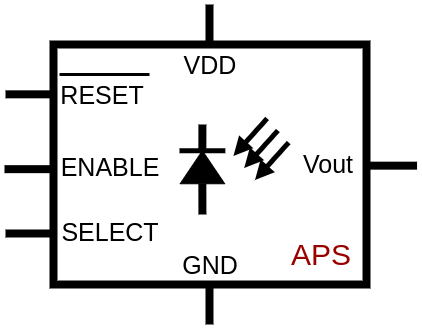
\includegraphics[scale=0.3]{Circuitos/APS_block.png}
    \legend{Fonte: Produzido pelo autor}
\end{figure}

Os transistores utilizados no bloco apresentam os par\^ametros mostrados na \autoref{\NomeTTab}. $W$ é a largura do canal. $L$ é o comprimento do canal $M$ representa o número de dispositivos em paralelo, enquanto $S$ representa o número de dispositivos em série.

\begin{table}[!h]
\caption{Transistores do bloco \NomeBloco}
\label{\NomeTTab}
\centering
\begin{tabular}{ccccc}
\toprule
Transistor & W ($\mu$m)  & L ($\mu$m)           & M (n° dispositivos) & S (n° dispositivos)\\
\midrule \midrule
T\textsubscript{buffer} & 15 & 0,75 & 1 & 1\\
\midrule
T\textsubscript{reset} & 4 & 0,18 & 1 & 1\\
\midrule
T\textsubscript{select} & 10 & 0,18 & 2 & 2\\
\bottomrule
\end{tabular}
\legend{Fonte: Produzido pelo autor}
\end{table}

O fotodiodo utilizado no bloco apresenta os par\^ametros mostrados na \autoref{\NomeQTab}. $W$ é a largura do fotodiodo. $L$ é o comprimento do fotodiodo.

\begin{table}[!h]
\caption{Fotodiodo do bloco \NomeBloco}
\label{\NomeQTab}
\centering
\begin{tabular}{ccccc}
\toprule
Nome & W ($\mu$m)  & L ($\mu$m)\\
\midrule \midrule
Fotodiodo & 25 & 25\\
\bottomrule
\end{tabular}
\legend{Fonte: Produzido pelo autor}
\end{table}

Informações referentes à $T\textsubscript{enable}$ podem ser vistas no \autoref{portatg}.